We now come to the running of the main two-stream and radiance code. The executable is {\tt l\_run\_cdl} for 
CDL input/output and {\tt l\_run\_cdf} for netCDF input/output. These can be run 
interactively, although it is usually more useful to run them from a UNIX script.

\section{UNIX command}

The UNIX-command is {\tt Cl\_run\_cdl} or {\tt Cl\_run\_cdf} which both take the same options.
The man page for {\tt Cl\_run\_cdf} follows formatted using {\tt man -t}.

\includepdf[pages=-]{Cl_run_cdf.pdf}

\subsection{Full Spectral Calculation}

The options required for using spherical harmonics to calculate radiances or fluxes are only
briefly dealt with in the man page. Explanation of these options is expanded here.

\begin{description}
\item [{\tt +S} {\it n1 n2 n3 n4} ] Calculate radiances by doing a full spectral calculation. 

\begin{description}
\item [{\it n1} ] Sets the type of truncation used with spherical harmonics, 
as defined in sph\_ truncation\_ pcf.f90: 1 triangular, 2 rhomboid, 3 symmetric.
\item [{\it n2} ] l-order of spherical harmonics.
\item [{\it n3} ] min m-order of spherical harmonics.
\item [{\it n4} ] max m-order of spherical harmonics.
\end{description}

The first issue to decide on is the truncation
of the infinite series of harmonics. In the IR there is no azimuthal
dependence, so we do not require non-axisymmetric terms with $m\neq 0$, for
which we select truncation 3 (the first number after +S). In the visible,
if radiances are required the truncation must be 1 to include non-axisymmetric
terms, but 3 can be used if only fluxes are required. The second number is
the order of truncation, which must be odd. The next two numbers specify
the azimuthal orders of truncation. For calculating fluxes, 
the two orders will be 0, but if calculating solar radiances the lowest
order would normally  be 0 and the highest equal to the global order of
truncation (but note that it is redundant to set it higher than the number
of non-zero terms in the phase function). Ocassionally, there might be a
need to examine particular ranges of azimuthal orders.

\item [{\tt -G} {\it basis truncation} ] Specify BRDF function to define surface
characteristics. BRDFs will be represented in the form
\begin{equation}
\gamma({\bf n}, {\bf n'})= \sum_{j=1}^N \rho_j F_j ({\bf n}, {\bf n'})
\end{equation}
where the $F_j$ are referred to as basis functions (this fits in with the
way in which models of BRDFs are often set up) and the $\rho_j$ are weights
which can vary from point to point. The number following the {\tt -G} specifies
the type of basis functions to be used, and at present must be 5 for a
Lambertian surface. The second number is the order of truncation of the
surface BRDF (which may be lower than that applied to the actual radiance
calculations if the BRDF is poorly characterized): in the case of Lambertian
surface this may clearly be 0. The $\rho_j$ are taken from the {\tt .surf} file,
and wherever sensible the $F_j$ will be normalised so that the $\rho_j$ will
be the albedo: this has been done for Lambertian surfaces. The file therefore
contains these weights for each basis function on the latitude-longitude
grid of the problem: the weights may vary from band to band, in which case
an extra dimension {\tt band} must be included in the file.

\end{description}

\noindent Arguments that can follow +S:

\begin{description}
\item [{\tt +F} ] Calculate fluxes rather than radiances.
\item [{\tt +P} ] Calculate photolysis rates rather than radiances.
\item [{\tt -H} ] Include the Heney-Greenstein approximation.
\item [{\tt -e} ] Use Euler transformation to improve convergence.
\item [{\tt -Y} ] Direct Calculation of Radiances.
\item [{\tt -T} ] Use the Iterative Source Function Technique. In general
better than -Y.
\item [{\tt -Z} {\it order} ] Specify the {\it order} of the solar truncation.
\end{description}

These options will benefit from further discussion. 
{\tt -H} requests Henyey-Greenstein phase functions. There are
several ways in which this could be interpreted, so it is well to discuss
what has been done. When Henyey-Greenstein phase functions are selected,
higher moments of each component are developed separately. More precisely,
the mean phase function is defined by
\begin{equation}
g_n= \sum_j k_j^{(s)} g_{j1}^n / \sum_j k_j^{(s)}
\end{equation}
where $k_j^{(s)}$ is the scattering extinction for the $j$th scattering
species, rather than as
\begin{equation}
g_n= \left (\sum_j k_j^{(s)} g_{j1} / \sum_j k_j^{(s)} \right )^n.
\end{equation}
The exception to this is Rayleigh scattering for which phase function
only $g_0$ and $g_2$ are non-zero: it does not seem sensible to extend
this as a Henyey-Greenstein phase function, so the true phase function
is always used. Henyey-Greenstein phase functions are also used indirectly.
Parametrizations used in the previous two-stream code give only asymmetries,
and it is convenient to extend these to full phase functions using a
Henyey-Greenstein approximation. It would thus be possible, say, to use
a fully calculated phase function for aerosols, but treat cloud droplets
using an old parametrization.

Some extra options are applicable when calculating radiances instead of
fluxes. {\bf -e} is helpful to improve convergence when the order of
truncation is more than, say 5 or so: the series giving the radiance
normally alternates and converges slowly, so convergence can be improved
by adding only half of the last term, which is the simplest form of Euler's
transformation. {\bf -Y} requests a direct calculation of radiances using
spherical harmonics. Usually, radiances should be calculated using the
iterative source function technique, selected by {\bf -T}. In the solar
region this can be trivially combined with the TMS-method of Nakajima and
Takano, calculaing the single scattering to a higher order: in this case
the order of solar truncation is specified by the option {\bf -Z}. Care
is required here. You can use a low overall order but a high order of
solar truncation only for radiances away from the solar direction; if
radiances in the aureole are required the overall order and the solar
order should both be set to high values (typically the same high value).

\section{Input files needed}

A vertical profile of temperature at the mid-points of layers ({\tt
.t}) will be needed as well as the temperatures at the edges of layers
({\tt .tl}), though the actual values are used only in the infrared
region; in the visible region this file merely defines the edges of
layers. At the surface the surface temperature {\tt .tstar} and the
surface pressure {\tt .pstar} are needed.  The latter is slightly
anomalous as it will only really be required when hybrid vertical
coordinates are implemented. In the solar region the solar zenith
angle {\tt .szen} and the irradiance at the TOA {\tt .stoa} are
needed, together with the azimuth {\tt .sazim} if calculating
radiances.  If you include gases, a file of mass mixing ratios must be
present for each gas in the spectral file, {\tt .q .co2} etc. Similarly, 
if you include aerosols a file of mass mixing ratios for each aerosol is
required. The file of surface characteristics {\tt .surf} has been discussed
above. If calculating radiances as opposed to fluxes, the polar and
azimuthal viewing angles as well as the viewing level must be
specified in a {\tt .view} file. When clouds are included a file of cloud 
fractions {\tt .clfr}, along with the mass mixing ratios of liquid water and 
ice, {\tt .lwm .iwm} and the effective radius of cloud droplets and ice-crystals, 
{\tt .re .ire}, are also required. Similar files are needed for the convective
cloud properties if these are included ({\tt -K} 3 or 4). The full list of file
suffixes can be found in the appendix.

\subsection{The {\tt .view} file}

This file specifies from which points and in which directions the radiances are 
to be output. The radiances can be calculated at a number of levels in the 
atmosphere. The floating point variable rlev is used to specify the viewing levels 
counting from the top of the atmosphere. For example:
{\small
\begin{verbatim}
             rlev =   .000000E+00,  .500000E+00;
\end{verbatim}
}
\noindent will provide radiances at the top of the atmosphere and halfway down 
the top layer.

\begin{figure}[htb]
\begin{center}
\latex{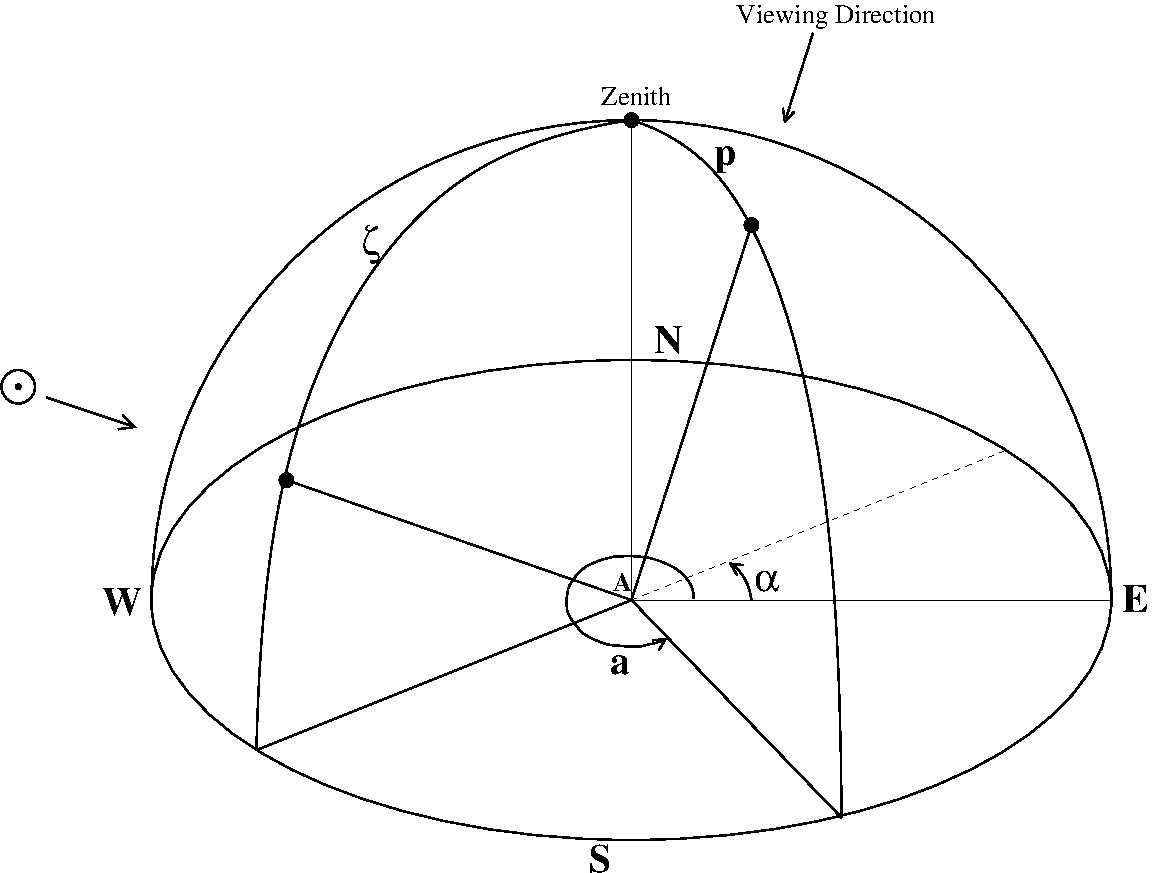
\includegraphics[width=14cm]{view.pdf}}
\html{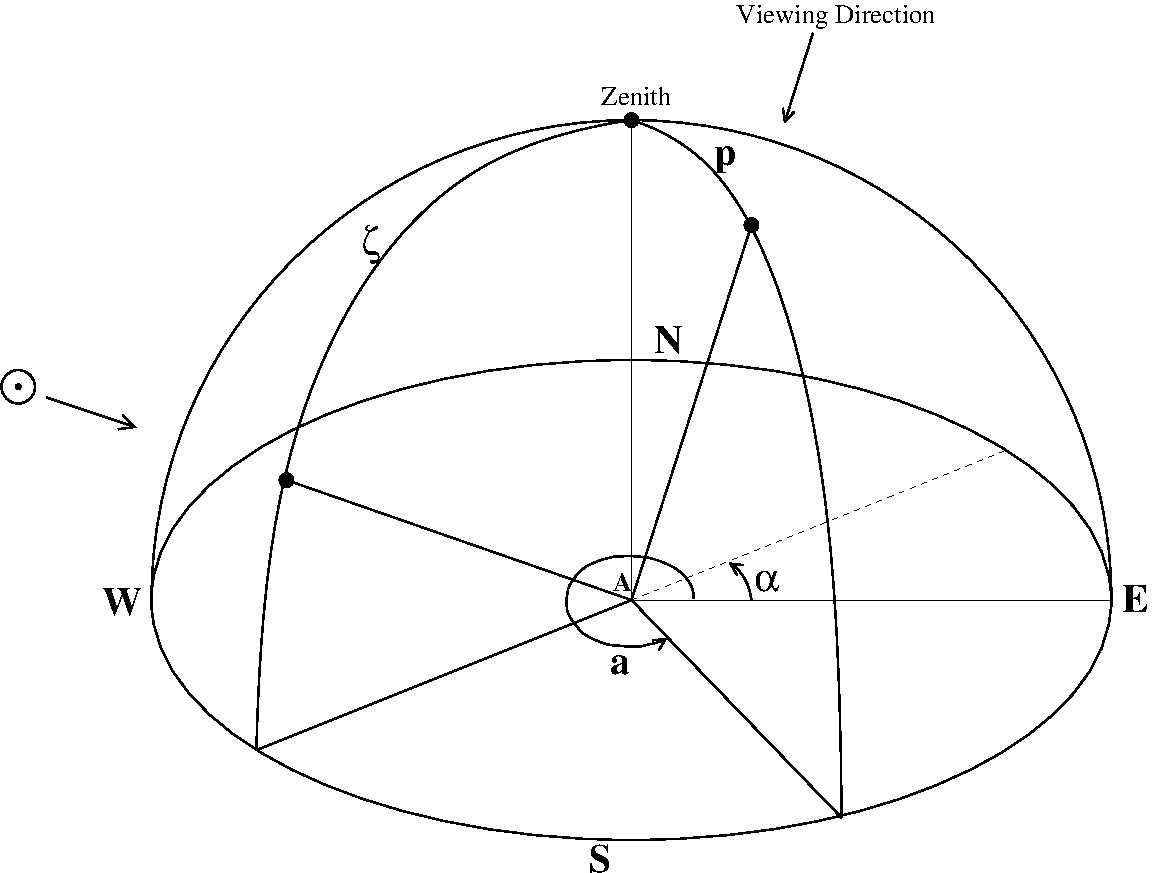
\includegraphics{view.gif}}
\caption{\label{fig:view} Specification of azimuthal and polar viewing angles for the output of radiances.
}
\end{center}
\end{figure}

For each viewing level, the viewing angles are specified in terms of an 
azimuthal and polar viewing angle. These are described most clearly with the 
aid of a diagram. Figure \ref{fig:view} displays the relevant angles from the perspective of point A on the surface. The sun (represented with a dotted circle) is in the south-west, with a solar zenith angle of $\zeta$. The solar azimuth angle represents the forward propogation direction of the solar beam, in this case angle $\alpha$. This has been defined in relation to a zero direction of due east (although the choice of zero direction is arbitrary). The viewing azimuth angle, {\it a} (azim in the {\tt .view} file), must be specified in relation to the same zero direction, anti-clockwise in the same manor as the solar azimuth angle. The viewing polar angle, {\it p} (pol in the {\tt .view} file), is specified in relation to the local zenith. A polar angle of 0 degrees indicates photons travelling straight up and would be applicable for a satellite passing directly overhead. A polar angle of 180 degrees indicates photons travelling straight down and would be applicable for an observer on the surface looking up.

An example {\tt .view} file can be seen in {\tt examples/rc3/rc3.view}.

\section{Using prescribed optical properties}

In the case of clouds and aerosols it is possible to use prescribed optical
properties on given levels. The setting up of a file containing such data is 
described in the previous chapter, but now it is time to discuss its application 
in the program. 

Starting with aerosols, the
option required is {\bf -a} and if this is specified alone the program will
expect to find files of mass mixing ratios on the usual grid (such as
{\tt .soot} for soot): parametrized data from the spectral file will be used.
If {\bf +A} is specified as well the program will first check for the
existence of files with suffixes consisting of the string {\tt op\_} followed
by that for the aerosol (such as {\tt .op\_soot}) which will be assumed to
contain the optical properties of the particular aerosol and these data will
be used instead of a parametrization. Prescribed profiles may be set for
only a selection of the aerosols in the spectral file. Within the program
optical properties will be required on the standard grid, but the levels
in the {\tt .op\_...} file do not have to match this. Using cubic splines,
the program will interpolate from the levels in the file of prescribed
properties to the midpoints of the layers, and will assume that the optical
properties are zero outside the specified range. An example may help. Suppose
that our grid consists of layers with mid-points every 50 mb moving up from
a surface pressure of 1000 mb. Perhaps we have a layer of soot aerosol between
620 and 830 mb, which we specify with optical properties at 630, 680, 730,
790 and 820 mb. In layers with mid-points at 600 mb and lower pressures, or
with mid-points at 850 mb and high pressures, it will be assumed that the
optical properties are zero. The values at 650--800 mb are calculated by
interpolation. There is a potential danger that interpolation may not
conserve the overall optical depth of the layer if the prescribed data are
coarsely resolved or inappropriately chosen: this must be borne in mind
when setting the data. 

The treatment of clouds is similar. To include
clouds we need {\bf -C} as mentioned above. When using prescribed optical
properties there is no need to include splits between convective and layer
cloud in the same grid-box, so we choose the simplest representation, {\bf
-K 1}. The program now expects to be given data for one type of water
droplets and/or one type of ice crystals. To include droplets we use the
option {\bf -d} followed by the type number and to include ice crystals
we use the option {\bf -i} followed by the type number. To use prescribed
profiles of optical properties these type numbers should be set to 0 or
a negative number. The program will then expect files with the suffix
{\tt .op\_water} or {\tt .op\_ice} containing the prescribed optical properties,
which will be interpolated as in the case of aerosols.

\section{Output files}

Output is given in netCDF/CDL files with the following suffixes:
.uflx (upward flux), .dflx (diffuse downward flux), .sflx (direct downward flux),
.vflx (total downward flux: dflx+sflx), .nflx (net downward flux: vflx-uflx),
.hrts (heating rates, K/day), .radn (radiance), .photol (rate of photolysis).
